\documentclass[a4paper,12pt]{article} 


\usepackage[T2A]{fontenc}			
\usepackage[utf8]{inputenc}			
\usepackage[english,russian]{babel}	

\usepackage{graphicx, scalerel}    
\usepackage{wrapfig}               
\usepackage[14pt]{extsizes}        
\usepackage[warn]{mathtext}       
\usepackage{indentfirst}      
\usepackage[margin = 25mm]{geometry}
\usepackage[table,xcdraw]{xcolor} 
\usepackage{amsmath,amsfonts,amssymb,amsthm,mathtools}
\usepackage{wasysym}                
\usepackage{upgreek}                
\usepackage{caption}
\usepackage{multirow}
\captionsetup{labelsep=period}
\usepackage[font=small,labelfont=bf]{caption}
\usepackage{gensymb}
\usepackage{icomma}

\usepackage[unicode, pdftex]{hyperref}
\usepackage{tikz}
\usetikzlibrary{positioning}
\usepackage{fancyhdr}
\pagestyle{fancy}
\setlength\fboxsep{3pt} % Отступ рамки \fbox{} от рисунка
\setlength\fboxrule{1pt} % Толщина линий рамки \fbox{}
\usepackage{tocloft}
\newcommand{\tocsection}[1]{\section*{#1} \addcontentsline{toc}{section}{#1}}
\renewcommand{\cftsecleader}{\cftdotfill{\cftdotsep}}


\begin{document}
	\newcommand{\HRule}{\rule{\linewidth}{0.7mm}} % Defines a new command for the horizontal lines, change thickness here

\begin{center}
	\large\textbf{Московский Физико-Технический Институт}\\
	\large\textbf{(государственный университет)}
	
	\vfill
	
	
	
	\Large Лабораторная работа 5.1.2
	%----------------------------------------------------------------------------------------
	%	TITLE SECTION
	%----------------------------------------------------------------------------------------
	
	\HRule
	\\[0.4cm]
	{ \huge \bfseries Исследование эффекта Комптона}
	\\[0.4cm] % Title of your document
	\HRule
	\\[0.5cm]
	
	\ \\
	\textbf{\large Автор:} \\	
	\large Овсянников Михаил Б01-008\\
	\vfill
	\hspace*{-0.8 cm}
\includegraphics[width=100 pt]{./Include/frkt_logo.pdf}\\
	\large Долгопрудный, 2022
\end{center}

\thispagestyle{empty}

\newpage
\setcounter{page}{2}
\fancyfoot[c]{\thepage}
\fancyhead[L] {Лабораторная работа 5.1.2}
\fancyhead[R] {Исследование эффекта Комптона}

	\newpage
	
	\tableofcontents
	
	
	
	\newpage
	\textbf{Цель работы:} методом электронного возбуждения измерить энергию первого уровня атома гелия в динамическом и статическом режимах.

	
	\tocsection{Теоретические сведения}
	
	\begin{wrapfigure}{R}{0.5\textwidth}
		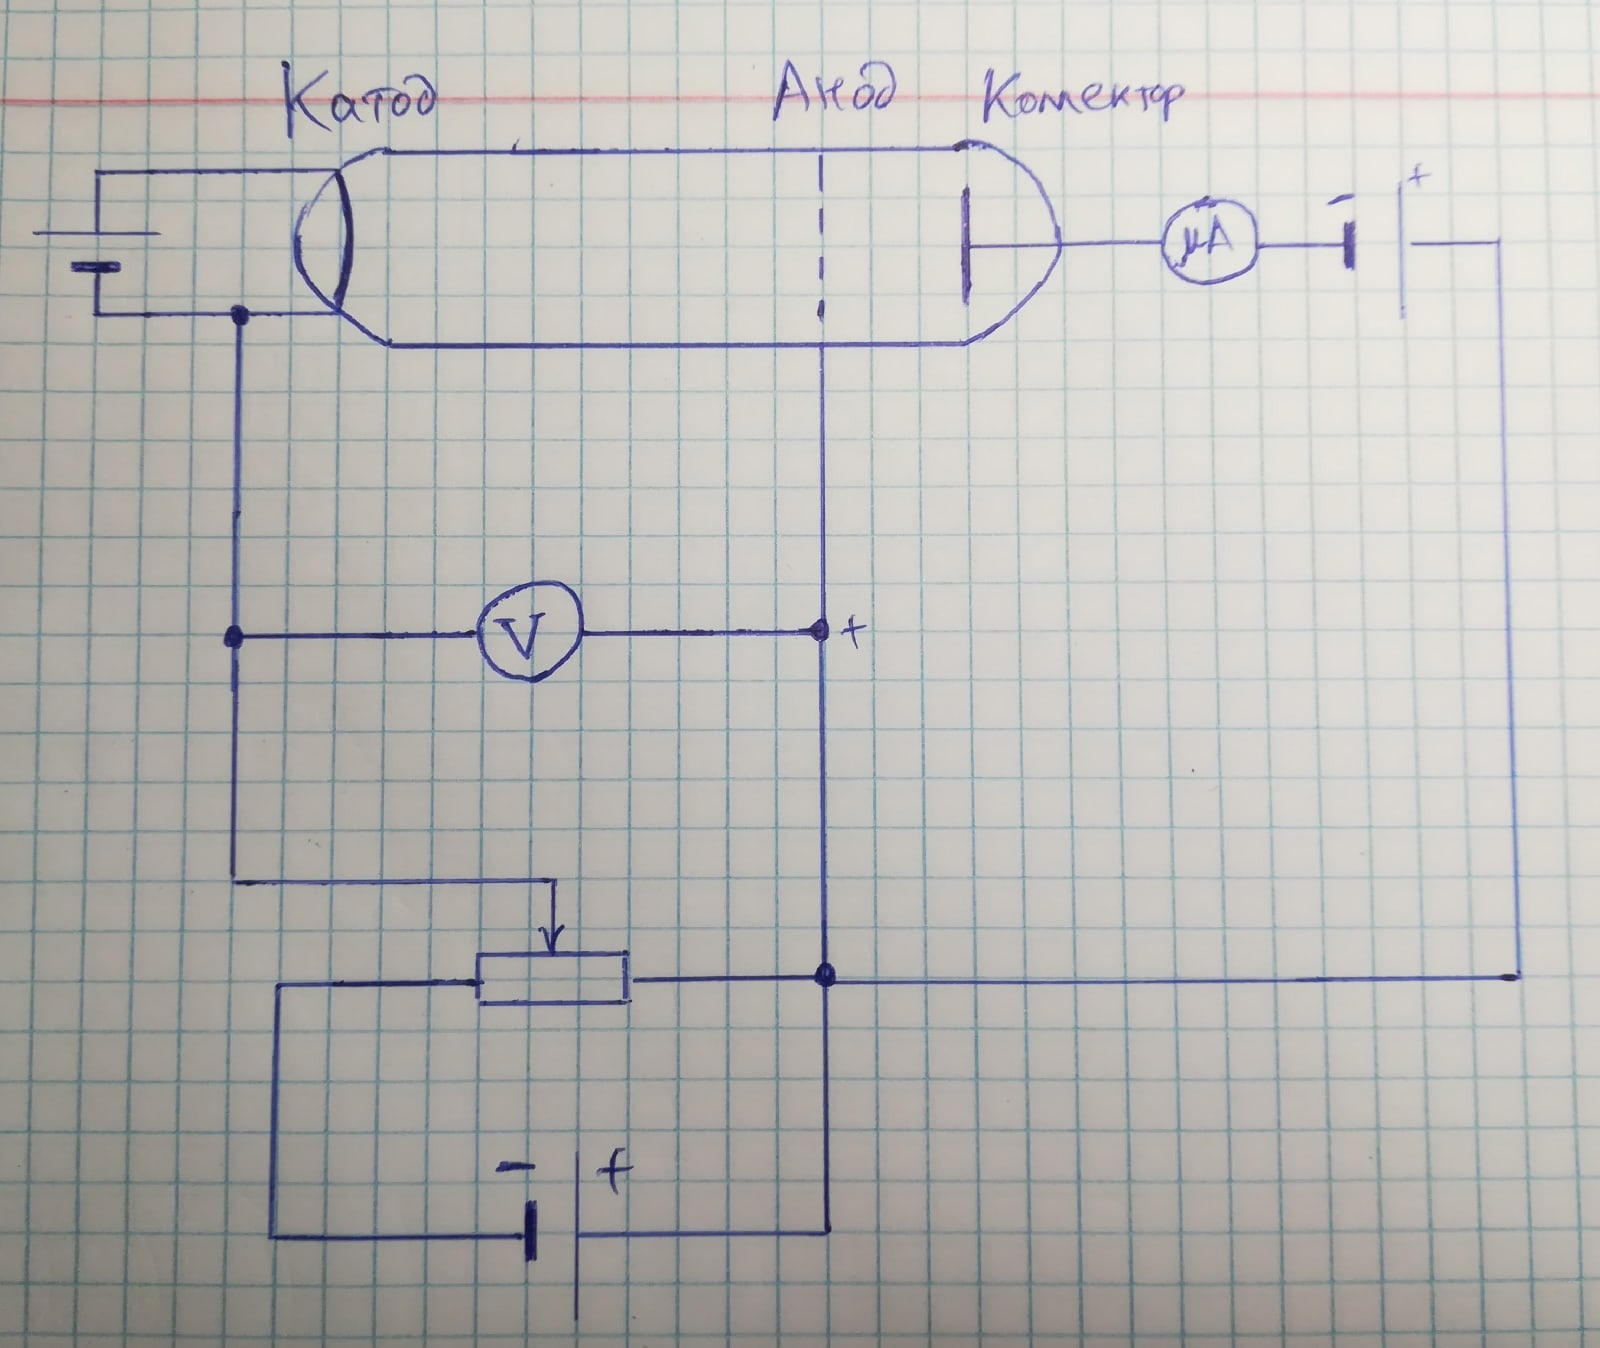
\includegraphics[width=0.5\textwidth]{./Pictures/Experiment.jpg}
		\caption{Схема опыта Франка и Герца}
		\label{Experiment}
	\end{wrapfigure}
	
	Одним из простых опытов, подтверждающих существование дискретных уровней энергии атомов, является эксперимент, известный под названием опыта Франка и Герца. Схема опыта изображена на рис. \ref{Experiment}.
	
	Разреженный одноатомный газ (в нашем случае — гелий) заполняет трехэлектродную лампу. Электроны, испускаемые разогретым катодом, ускоряются в постоянном электрическом поле, созданном между катодом и сетчатым анодом лампы и сталкиваются с атомами гелия. Если энергия электрона, налетающего на атом, недостаточна для того, чтобы перевести его в возбужденное состояние, то возможны только упругие соударения.
	
	По мере увеличения разности потенциалов между анодом и катодом энергия электронов увеличивается и, в конце концов, оказывается достаточной для возбуждения атомов. При таких -- неупругих -- столкновениях кинетическая энергия налетающего электрона передается одному из атомных электронов, вызывая его переход на свободный энергетический уровень (возбуждение) или совсем отрывая его от атома (ионизация).
	
	Ток коллектора, пропорциональный числу электронов, попадающих на него за секунду, измеряется микроамперметром.

	
	При увеличении потенциала анода ток в лампе вначале растет. Однако, когда энергия электронов становится достаточной для возбуждения атомов, ток коллектора резко уменьшается. При дальнейшем увеличении потенциала анода ток коллектора вновь возрастает.

	
	Следующее замедление роста тока происходит в момент, когда часть
	электронов неупруго сталкивается с атомами два раза: первый раз посередине пути, второй -- у анода и т. д. Таким образом, на кривой зависимости тока коллектора от напряжения анода имеется ряд максимумов и минимумов, отстоящих друг от друга на равные расстояния $\Delta V$. Эти расстояния равны энергии первого возбужденного состояния.
	
	\tocsection{Экспериментальная установка}
	
	\begin{wrapfigure}{L}{0.5\textwidth}
		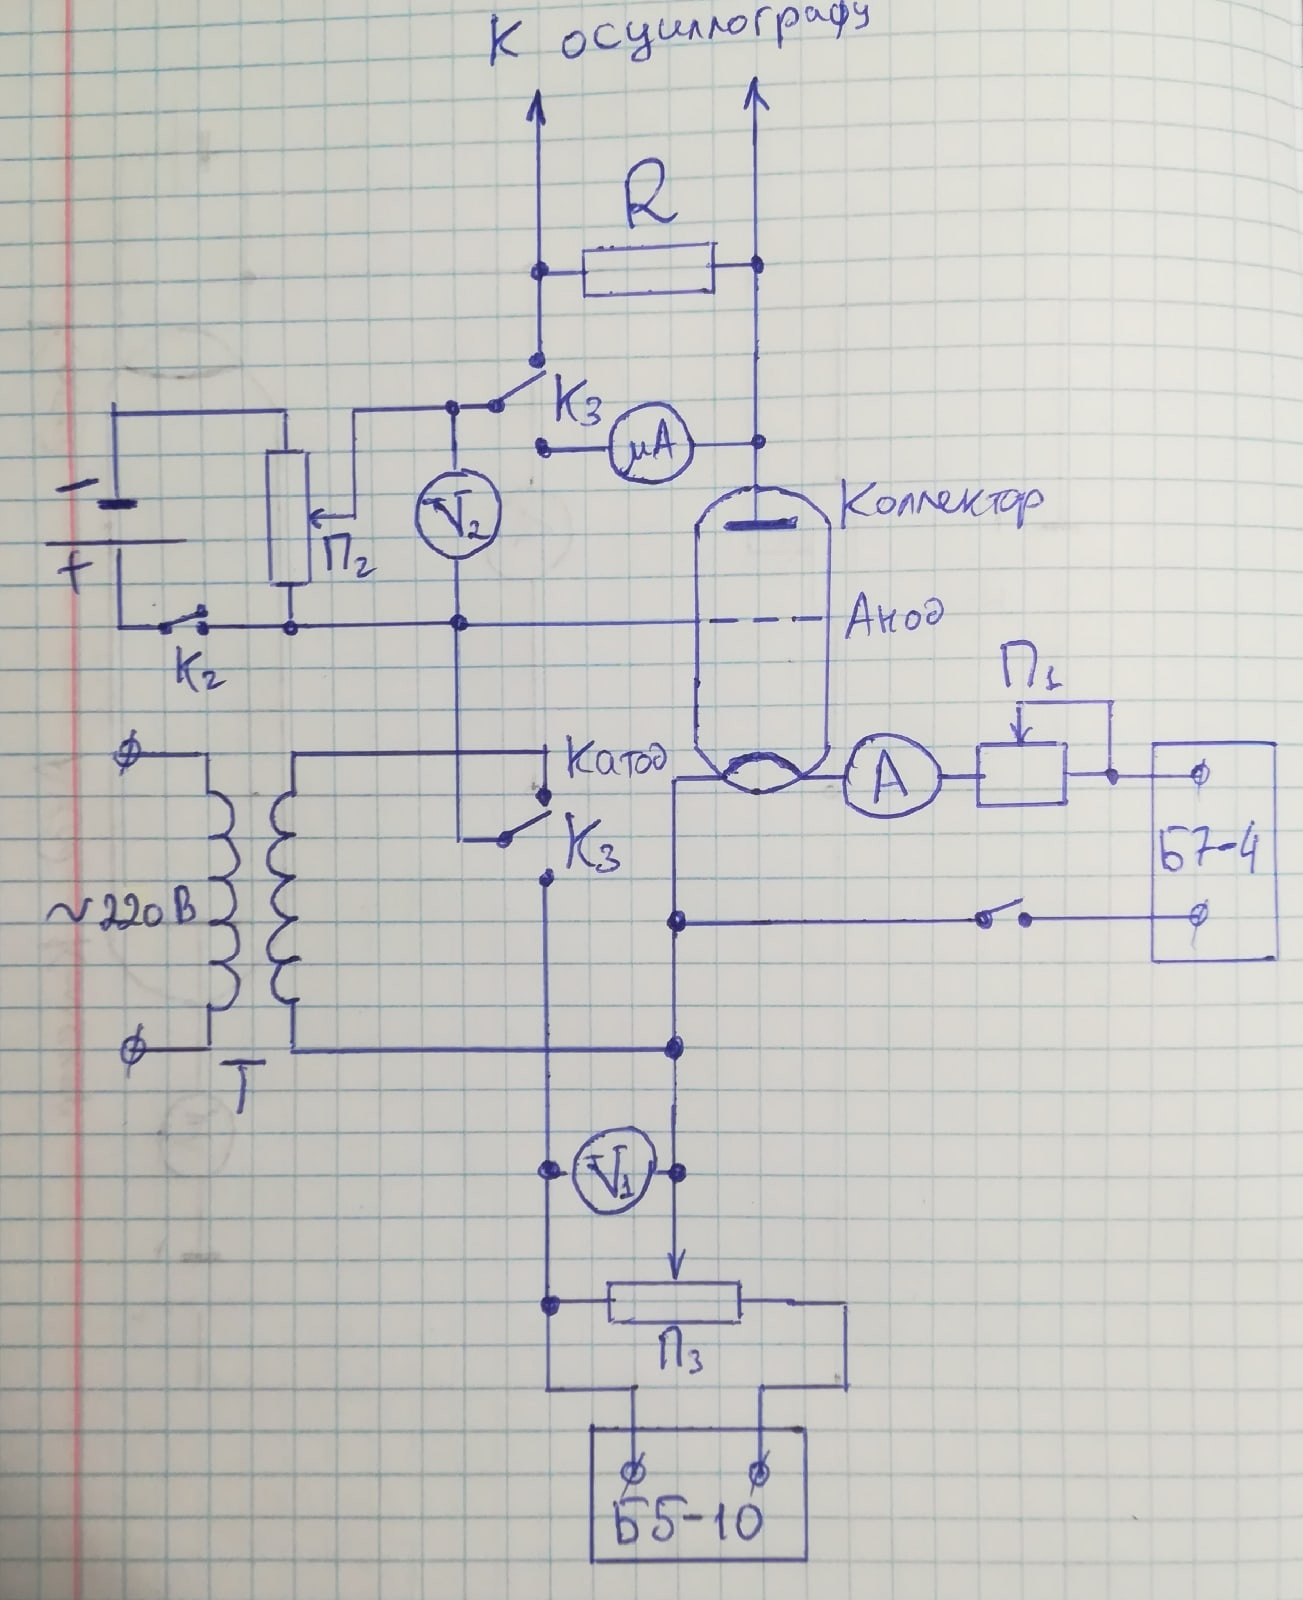
\includegraphics[width=0.5\textwidth]{./Pictures/Circuit.jpg}
		\caption{Схема экспериментальной установки}
		\label{Circuit}
	\end{wrapfigure}

	
	Схема экспериментальной установки изображена на рис. \ref{Circuit}. Для опыта используется серийная лампа ионизационного манометра ЛМ-2, заполненная гелием. Напряжение накала подается от стабилизированного источника питания Б7-4. Ток накала контролируется амперметром А. Источник Б7-4 включается в цепь тумблером К$_1$.
	
	В качестве анода используется двойная спираль, окружающая катод. Роль коллектора играет полый металлический цилиндр, соосный с катодом и анодом.
	
	Ускоряющее напряжение подается на анод от выпрямителя Б5-10. Величина этого напряжения регулируется потенциометром П$_3$ и измеряется вольтметром $V_1$. Источник задерживающего потенциала -- батарея КБСЛ (4,5 В) -- включается ключом K$_2$, величина потенциала регулируется потенциометром П$_2$ и измеряется вольтметром $V_2$. Ток в цепи коллектора регистрируется микроамперметром.

	Схему можно переключать из статического режима измерений в динамический режим с помощью ключа K$_3$. На рис. \ref{Circuit} две части сдвоенного ключа K$_3$ изображены отдельно. При динамическом режиме работы ускоряющий потенциал подается с понижающего трансформатора $T$ (220/50 В), а ток коллектора регистрируется осциллографом, подключенным к нагрузочному резистору $R$. Осциллограф следует синхронизировать от сети 50 Гц.

	
	При определении энергии электронов по разности потенциалов между анодом и катодом следует иметь в виду, что из-за контактной разности потенциалов между катодом и анодом первый максимум не соответствует потенциалу первого возбужденного уровня. Однако контактная разность потенциалов так сдвигает все максимумы, что расстояние между ними не меняется.
	
	\newpage
	

	\tocsection{Ход работы}
	
	\subsection*{Подготовка приборов к работе}
	\addcontentsline{toc}{subsection}{Подготовка приборов к работе}
	

	\begin{enumerate}
		\item Установим все ручки на источнике питания в крайнее левое положение и включим прибор в сеть.
		
		\item Включим электронный осциллограф в сеть.
		
		\item На канале I, измеряющем анодное напряжение лампы, установим ступенчатый переключатель в положение 1 V/дел, утопим соседнюю кнопку $\times 10$.
		
		\item На канале II, измеряющем напряжение, пропорциональное току коллектора лампы, установим переключатель в положение 2 mV/дел, кнопку $\times 10$ вытянем на себя.
		
		\item Утопим клавиши <<x-y>> слева и справа от экрана осциллографа.
 	\end{enumerate}
 	
 	\subsection*{Получение ВАХ $I_k = f(V_a)$ на экране осциллографа С1-83}
 	\addcontentsline{toc}{subsection}{Получение ВАХ $I_k = f(V_a)$ на экране осциллографа С1-83}

 
 	\begin{enumerate}
 		\item Установим динамический режим.
 		
 		\item Установим задерживающее напряжение 4 В.
 		
 		\item Установим ручку накала на максимум.
 		
 		\item Проследим за ходом ВАХ при изменении ускоряющего напряжения (рис. \ref{Dynamic}).
 		
 		\item Разместим картину в центре экрана осциллографа.
 		
 		\item При максимальном ускоряющем напряжении измерим на экране расстояния между максимума и минимумами осциллограммы. Проведем такие измерения для 3-х значений задерживающего напряжения: 4, 6 и 8 В. Результаты пишем в таблицу \ref{MaxMin}.
 		
 		\item Прежде, чем перейти к измерениям в статическом режиме, выключим осциллограф.
 		
 		\newpage
 		
 		\begin{figure}[h!]
 			\centering
 			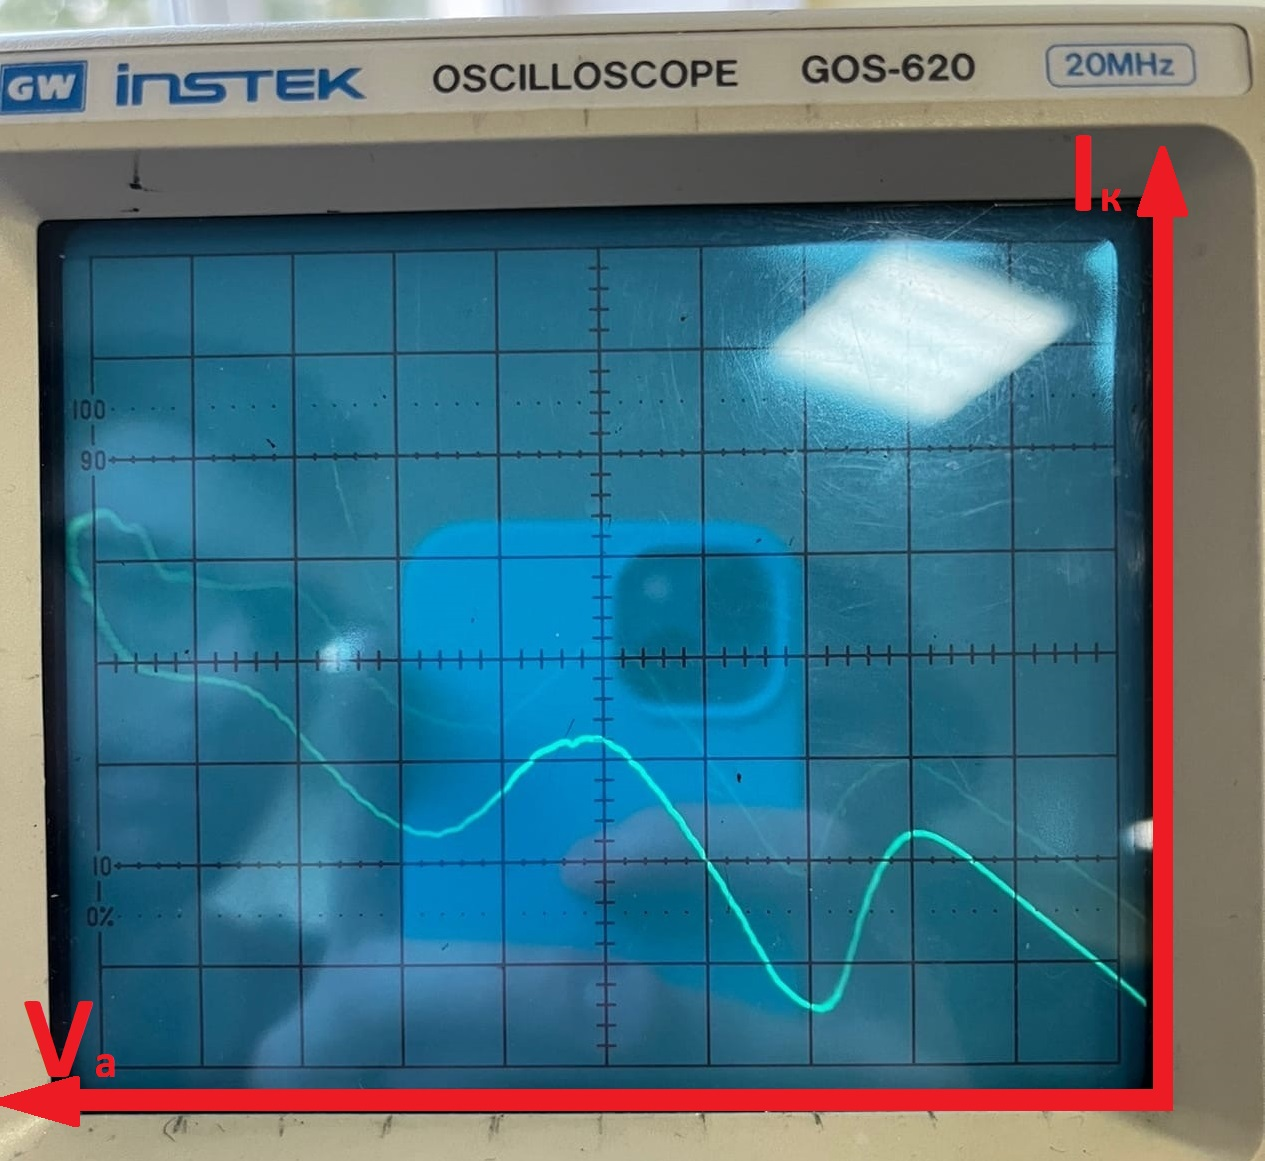
\includegraphics[width=\linewidth]{./Pictures/Pic1.jpg}
 			\caption{ВАХ на экране осциллографа}
 			\label{Dynamic}
 		\end{figure}
 	\end{enumerate}
 
 	\subsection*{Получение ВАХ $I_k = f(V_a)$ в статическом режиме измерений}
 	\addcontentsline{toc}{subsection}{Получение ВАХ $I_k = f(V_a)$ в статическом режиме измерений}

 
 	\begin{enumerate}
 		\item Переведем режим в статический
 		
 		\item Установим максимальный накал и задерживающее напряжение на 4 В.
 		
 		\item Включим микроамперметр и вольтметр.
 		
 		\item Снимем зависимость коллекторного тока от анодного напряжения $I_\text{к} = f(V_a)$ для 3-х различных значений задерживающего напряжения $V_2 = 4, \; 6, \; 8$ В. Результаты занесем в таблицу \ref{Static}.
 		
 		\item Закончив работу, отключим все приборы.
 	\end{enumerate}
 
 	\newpage
 	
 	\subsection*{Обработка результатов}
 	\addcontentsline{toc}{subsection}{Обработка результатов}
 	
 	\begin{enumerate}
 		\item По расстоянию между соседними максимумами на осциллограммах определим энергию возбуждения первого уровня атома гелия.
 		
 	
 		\begin{table}[h!]
 			\centering
 			\begin{tabular}{|c|c|c|}
 				\hline
 				$V_\text{задерж}$, В & $\Delta V_\text{max}$, В & $\Delta V_\text{min}$, В \\ \hline
 				\multirow{2}{*}{4}   & 14                       & 17                       \\ \cline{2-3} 
 				& 15                       & 12                       \\ \hline
 				\multirow{2}{*}{6}   & 15                       & 18                       \\ \cline{2-3} 
 				& 16                       & 13                       \\ \hline
 				\multirow{2}{*}{8}   & 14                       & 19                       \\ \cline{2-3} 
 				& 15                       & 12                       \\ \hline
 			\end{tabular}
 			\caption{Расстояние между максимумами и расстояние между минимумами в динамическом режиме. Погрешность измерения каждого напряжения $\sigma_V = 1 $ В}
 			\label{MaxMin}
 		\end{table}
 		
 		
 		Тогда среднее значение:
 		
 		\begin{equation*}
 			\Delta V = (15,0 \pm 3,5) \text{ В} \hspace{20mm} (\text{погрешность}\thicksim 23 \% )
 		\end{equation*}
 	
 		То есть энергия возбуждения первого уровня атома гелия:
 		\begin{equation*}
 			E_1 = (15,0 \pm 3,5) \text{ эВ} \hspace{20mm} (\text{погрешность}\thicksim 23 \% )
 		\end{equation*}
 		
 		
 		\item По результатам таблицы \ref{Static} построим графики зависимостей $I_\text{к} = f(V_a)$ для трех значений задерживающего напряжения.
 		
 		\newpage
 		
 		\begin{table}[h!]
 			\centering
 			\scalebox{0.8}{
				\begin{tabular}{|cc|cccccccccccccccc}
					\cline{1-2} \cline{9-10} \cline{17-18}
					\multicolumn{2}{|c|}{$V_\text{задерж} = 4$ В}      &  &  &  &  &  & \multicolumn{1}{c|}{} & \multicolumn{2}{c|}{$V_\text{задерж} = 6$ В}                           &  &  &  &  &  & \multicolumn{1}{c|}{} & \multicolumn{2}{c|}{$V_\text{задерж} = 8$ В}                           \\ \cline{1-2} \cline{9-10} \cline{17-18} 
					\multicolumn{1}{|c|}{$V_a$, В} & $I_\text{к}$, мкА &  &  &  &  &  & \multicolumn{1}{c|}{} & \multicolumn{1}{c|}{$V_a$, В} & \multicolumn{1}{c|}{$I_\text{к}$, мкА} &  &  &  &  &  & \multicolumn{1}{c|}{} & \multicolumn{1}{c|}{$V_a$, В} & \multicolumn{1}{c|}{$I_\text{к}$, мкА} \\ \cline{1-2} \cline{9-10} \cline{17-18} 
					\multicolumn{1}{|c|}{2,95}     & 28                &  &  &  &  &  & \multicolumn{1}{c|}{} & \multicolumn{1}{c|}{2,35}     & \multicolumn{1}{c|}{13}                &  &  &  &  &  & \multicolumn{1}{c|}{} & \multicolumn{1}{c|}{5,94}     & \multicolumn{1}{c|}{17}                \\ \cline{1-2} \cline{9-10} \cline{17-18} 
					\multicolumn{1}{|c|}{3,65}     & 32                &  &  &  &  &  & \multicolumn{1}{c|}{} & \multicolumn{1}{c|}{4,22}     & \multicolumn{1}{c|}{22}                &  &  &  &  &  & \multicolumn{1}{c|}{} & \multicolumn{1}{c|}{9,25}     & \multicolumn{1}{c|}{40}                \\ \cline{1-2} \cline{9-10} \cline{17-18} 
					\multicolumn{1}{|c|}{4,55}     & 38                &  &  &  &  &  & \multicolumn{1}{c|}{} & \multicolumn{1}{c|}{5,76}     & \multicolumn{1}{c|}{32}                &  &  &  &  &  & \multicolumn{1}{c|}{} & \multicolumn{1}{c|}{12,23}    & \multicolumn{1}{c|}{69}                \\ \cline{1-2} \cline{9-10} \cline{17-18} 
					\multicolumn{1}{|c|}{6,33}     & 53                &  &  &  &  &  & \multicolumn{1}{c|}{} & \multicolumn{1}{c|}{6,44}     & \multicolumn{1}{c|}{36}                &  &  &  &  &  & \multicolumn{1}{c|}{} & \multicolumn{1}{c|}{13,79}    & \multicolumn{1}{c|}{81}                \\ \cline{1-2} \cline{9-10} \cline{17-18} 
					\multicolumn{1}{|c|}{7,18}     & 60                &  &  &  &  &  & \multicolumn{1}{c|}{} & \multicolumn{1}{c|}{8,58}     & \multicolumn{1}{c|}{55}                &  &  &  &  &  & \multicolumn{1}{c|}{} & \multicolumn{1}{c|}{15,30}    & \multicolumn{1}{c|}{93}                \\ \cline{1-2} \cline{9-10} \cline{17-18} 
					\multicolumn{1}{|c|}{8,24}     & 68                &  &  &  &  &  & \multicolumn{1}{c|}{} & \multicolumn{1}{c|}{9,71}     & \multicolumn{1}{c|}{64}                &  &  &  &  &  & \multicolumn{1}{c|}{} & \multicolumn{1}{c|}{16,33}    & \multicolumn{1}{c|}{101}               \\ \cline{1-2} \cline{9-10} \cline{17-18} 
					\multicolumn{1}{|c|}{9,94}     & 81                &  &  &  &  &  & \multicolumn{1}{c|}{} & \multicolumn{1}{c|}{11,42}    & \multicolumn{1}{c|}{77}                &  &  &  &  &  & \multicolumn{1}{c|}{} & \multicolumn{1}{c|}{18,22}    & \multicolumn{1}{c|}{116}               \\ \cline{1-2} \cline{9-10} \cline{17-18} 
					\multicolumn{1}{|c|}{11,37}    & 91                &  &  &  &  &  & \multicolumn{1}{c|}{} & \multicolumn{1}{c|}{13,88}    & \multicolumn{1}{c|}{96}                &  &  &  &  &  & \multicolumn{1}{c|}{} & \multicolumn{1}{c|}{20,41}    & \multicolumn{1}{c|}{126}               \\ \cline{1-2} \cline{9-10} \cline{17-18} 
					\multicolumn{1}{|c|}{13,52}    & 107               &  &  &  &  &  & \multicolumn{1}{c|}{} & \multicolumn{1}{c|}{16,02}    & \multicolumn{1}{c|}{114}               &  &  &  &  &  & \multicolumn{1}{c|}{} & \multicolumn{1}{c|}{20,57}    & \multicolumn{1}{c|}{127}               \\ \cline{1-2} \cline{9-10} \cline{17-18} 
					\multicolumn{1}{|c|}{15,17}    & 118               &  &  &  &  &  & \multicolumn{1}{c|}{} & \multicolumn{1}{c|}{17,61}    & \multicolumn{1}{c|}{125}               &  &  &  &  &  & \multicolumn{1}{c|}{} & \multicolumn{1}{c|}{22,76}    & \multicolumn{1}{c|}{119}               \\ \cline{1-2} \cline{9-10} \cline{17-18} 
					\multicolumn{1}{|c|}{16,61}    & 128               &  &  &  &  &  & \multicolumn{1}{c|}{} & \multicolumn{1}{c|}{19,34}    & \multicolumn{1}{c|}{135}               &  &  &  &  &  & \multicolumn{1}{c|}{} & \multicolumn{1}{c|}{23,36}    & \multicolumn{1}{c|}{105}               \\ \cline{1-2} \cline{9-10} \cline{17-18} 
					\multicolumn{1}{|c|}{18,05}    & 137               &  &  &  &  &  & \multicolumn{1}{c|}{} & \multicolumn{1}{c|}{19,97}    & \multicolumn{1}{c|}{137}               &  &  &  &  &  & \multicolumn{1}{c|}{} & \multicolumn{1}{c|}{23,59}    & \multicolumn{1}{c|}{100}               \\ \cline{1-2} \cline{9-10} \cline{17-18} 
					\multicolumn{1}{|c|}{18,77}    & 141               &  &  &  &  &  & \multicolumn{1}{c|}{} & \multicolumn{1}{c|}{20,62}    & \multicolumn{1}{c|}{136}               &  &  &  &  &  & \multicolumn{1}{c|}{} & \multicolumn{1}{c|}{23,86}    & \multicolumn{1}{c|}{41}                \\ \cline{1-2} \cline{9-10} \cline{17-18} 
					\multicolumn{1}{|c|}{19,83}    & 142               &  &  &  &  &  & \multicolumn{1}{c|}{} & \multicolumn{1}{c|}{21,31}    & \multicolumn{1}{c|}{134}               &  &  &  &  &  & \multicolumn{1}{c|}{} & \multicolumn{1}{c|}{23,94}    & \multicolumn{1}{c|}{39}                \\ \cline{1-2} \cline{9-10} \cline{17-18} 
					\multicolumn{1}{|c|}{20,42}    & 140               &  &  &  &  &  & \multicolumn{1}{c|}{} & \multicolumn{1}{c|}{22,67}    & \multicolumn{1}{c|}{117}               &  &  &  &  &  & \multicolumn{1}{c|}{} & \multicolumn{1}{c|}{24,44}    & \multicolumn{1}{c|}{28}                \\ \cline{1-2} \cline{9-10} \cline{17-18} 
					\multicolumn{1}{|c|}{20,82}    & 137               &  &  &  &  &  & \multicolumn{1}{c|}{} & \multicolumn{1}{c|}{23,30}    & \multicolumn{1}{c|}{88}                &  &  &  &  &  & \multicolumn{1}{c|}{} & \multicolumn{1}{c|}{25,69}    & \multicolumn{1}{c|}{15}                \\ \cline{1-2} \cline{9-10} \cline{17-18} 
					\multicolumn{1}{|c|}{21,53}    & 131               &  &  &  &  &  & \multicolumn{1}{c|}{} & \multicolumn{1}{c|}{23,79}    & \multicolumn{1}{c|}{41}                &  &  &  &  &  & \multicolumn{1}{c|}{} & \multicolumn{1}{c|}{26,49}    & \multicolumn{1}{c|}{12}                \\ \cline{1-2} \cline{9-10} \cline{17-18} 
					\multicolumn{1}{|c|}{22,14}    & 123               &  &  &  &  &  & \multicolumn{1}{c|}{} & \multicolumn{1}{c|}{24,24}    & \multicolumn{1}{c|}{35}                &  &  &  &  &  & \multicolumn{1}{c|}{} & \multicolumn{1}{c|}{27,52}    & \multicolumn{1}{c|}{14}                \\ \cline{1-2} \cline{9-10} \cline{17-18} 
					\multicolumn{1}{|c|}{23,01}    & 77                &  &  &  &  &  & \multicolumn{1}{c|}{} & \multicolumn{1}{c|}{25,08}    & \multicolumn{1}{c|}{33}                &  &  &  &  &  & \multicolumn{1}{c|}{} & \multicolumn{1}{c|}{28,95}    & \multicolumn{1}{c|}{23}                \\ \cline{1-2} \cline{9-10} \cline{17-18} 
					\multicolumn{1}{|c|}{23,61}    & 65                &  &  &  &  &  & \multicolumn{1}{c|}{} & \multicolumn{1}{c|}{25,62}    & \multicolumn{1}{c|}{35}                &  &  &  &  &  & \multicolumn{1}{c|}{} & \multicolumn{1}{c|}{30,29}    & \multicolumn{1}{c|}{36}                \\ \cline{1-2} \cline{9-10} \cline{17-18} 
					\multicolumn{1}{|c|}{24,81}    & 67                &  &  &  &  &  & \multicolumn{1}{c|}{} & \multicolumn{1}{c|}{27,82}    & \multicolumn{1}{c|}{54}                &  &  &  &  &  & \multicolumn{1}{c|}{} & \multicolumn{1}{c|}{32,50}    & \multicolumn{1}{c|}{71}                \\ \cline{1-2} \cline{9-10} \cline{17-18} 
					\multicolumn{1}{|c|}{26,38}    & 87                &  &  &  &  &  & \multicolumn{1}{c|}{} & \multicolumn{1}{c|}{29,46}    & \multicolumn{1}{c|}{78}                &  &  &  &  &  & \multicolumn{1}{c|}{} & \multicolumn{1}{c|}{33,90}    & \multicolumn{1}{c|}{92}                \\ \cline{1-2} \cline{9-10} \cline{17-18} 
					\multicolumn{1}{|c|}{27,82}    & 108               &  &  &  &  &  & \multicolumn{1}{c|}{} & \multicolumn{1}{c|}{30,66}    & \multicolumn{1}{c|}{96}                &  &  &  &  &  & \multicolumn{1}{c|}{} & \multicolumn{1}{c|}{35,24}    & \multicolumn{1}{c|}{109}               \\ \cline{1-2} \cline{9-10} \cline{17-18} 
					\multicolumn{1}{|c|}{28,77}    & 121               &  &  &  &  &  & \multicolumn{1}{c|}{} & \multicolumn{1}{c|}{32,06}    & \multicolumn{1}{c|}{115}               &  &  &  &  &  & \multicolumn{1}{c|}{} & \multicolumn{1}{c|}{37,53}    & \multicolumn{1}{c|}{119}               \\ \cline{1-2} \cline{9-10} \cline{17-18} 
					\multicolumn{1}{|c|}{29,56}    & 131               &  &  &  &  &  & \multicolumn{1}{c|}{} & \multicolumn{1}{c|}{33,96}    & \multicolumn{1}{c|}{140}               &  &  &  &  &  & \multicolumn{1}{c|}{} & \multicolumn{1}{c|}{38,47}    & \multicolumn{1}{c|}{121}               \\ \cline{1-2} \cline{9-10} \cline{17-18} 
					\multicolumn{1}{|c|}{30,66}    & 145               &  &  &  &  &  & \multicolumn{1}{c|}{} & \multicolumn{1}{c|}{35,29}    & \multicolumn{1}{c|}{155}               &  &  &  &  &  & \multicolumn{1}{c|}{} & \multicolumn{1}{c|}{40,07}    & \multicolumn{1}{c|}{112}               \\ \cline{1-2} \cline{9-10} \cline{17-18} 
					\multicolumn{1}{|c|}{31,25}    & 153               &  &  &  &  &  & \multicolumn{1}{c|}{} & \multicolumn{1}{c|}{37,06}    & \multicolumn{1}{c|}{161}               &  &  &  &  &  & \multicolumn{1}{c|}{} & \multicolumn{1}{c|}{41,90}    & \multicolumn{1}{c|}{101}               \\ \cline{1-2} \cline{9-10} \cline{17-18} 
					\multicolumn{1}{|c|}{32,58}    & 168               &  &  &  &  &  & \multicolumn{1}{c|}{} & \multicolumn{1}{c|}{38,42}    & \multicolumn{1}{c|}{162}               &  &  &  &  &  & \multicolumn{1}{c|}{} & \multicolumn{1}{c|}{44,07}    & \multicolumn{1}{c|}{89}                \\ \cline{1-2} \cline{9-10} \cline{17-18} 
					\multicolumn{1}{|c|}{32,74}    & 171               &  &  &  &  &  & \multicolumn{1}{c|}{} & \multicolumn{1}{c|}{39,33}    & \multicolumn{1}{c|}{158}               &  &  &  &  &  & \multicolumn{1}{c|}{} & \multicolumn{1}{c|}{46,83}    & \multicolumn{1}{c|}{71}                \\ \cline{1-2} \cline{9-10} \cline{17-18} 
					\multicolumn{1}{|c|}{34,12}    & 187               &  &  &  &  &  & \multicolumn{1}{c|}{} & \multicolumn{1}{c|}{41,96}    & \multicolumn{1}{c|}{138}               &  &  &  &  &  & \multicolumn{1}{c|}{} & \multicolumn{1}{c|}{48,95}    & \multicolumn{1}{c|}{62}                \\ \cline{1-2} \cline{9-10} \cline{17-18} 
					\multicolumn{1}{|c|}{35,54}    & 200               &  &  &  &  &  & \multicolumn{1}{c|}{} & \multicolumn{1}{c|}{44,39}    & \multicolumn{1}{c|}{122}               &  &  &  &  &  & \multicolumn{1}{c|}{} & \multicolumn{1}{c|}{51,06}    & \multicolumn{1}{c|}{59}                \\ \cline{1-2} \cline{9-10} \cline{17-18} 
					\multicolumn{1}{|c|}{36,29}    & 202               &  &  &  &  &  & \multicolumn{1}{c|}{} & \multicolumn{1}{c|}{46,13}    & \multicolumn{1}{c|}{114}               &  &  &  &  &  & \multicolumn{1}{c|}{} & \multicolumn{1}{c|}{52,86}    & \multicolumn{1}{c|}{63}                \\ \cline{1-2} \cline{9-10} \cline{17-18} 
					\multicolumn{1}{|c|}{37,18}    & 201               &  &  &  &  &  & \multicolumn{1}{c|}{} & \multicolumn{1}{c|}{47,80}    & \multicolumn{1}{c|}{110}               &  &  &  &  &  & \multicolumn{1}{c|}{} & \multicolumn{1}{c|}{55,36}    & \multicolumn{1}{c|}{75}                \\ \cline{1-2} \cline{9-10} \cline{17-18} 
					\multicolumn{1}{|c|}{37,83}    & 201               &  &  &  &  &  & \multicolumn{1}{c|}{} & \multicolumn{1}{c|}{50,67}    & \multicolumn{1}{c|}{115}               &  &  &  &  &  & \multicolumn{1}{c|}{} & \multicolumn{1}{c|}{59,75}    & \multicolumn{1}{c|}{91}                \\ \cline{1-2} \cline{9-10} \cline{17-18} 
					\multicolumn{1}{|c|}{40,18}    & 187               &  &  &  &  &  & \multicolumn{1}{c|}{} & \multicolumn{1}{c|}{52,09}    & \multicolumn{1}{c|}{120}               &  &  &  &  &  & \multicolumn{1}{c|}{} & \multicolumn{1}{c|}{63,64}    & \multicolumn{1}{c|}{94}                \\ \cline{1-2} \cline{9-10} \cline{17-18} 
					\multicolumn{1}{|c|}{41,86}    & 174               &  &  &  &  &  & \multicolumn{1}{c|}{} & \multicolumn{1}{c|}{54,54}    & \multicolumn{1}{c|}{134}               &  &  &  &  &  & \multicolumn{1}{c|}{} & \multicolumn{1}{c|}{66,85}    & \multicolumn{1}{c|}{89}                \\ \cline{1-2} \cline{9-10} \cline{17-18} 
					\multicolumn{1}{|c|}{42,85}    & 169               &  &  &  &  &  & \multicolumn{1}{c|}{} & \multicolumn{1}{c|}{57,86}    & \multicolumn{1}{c|}{153}               &  &  &  &  &  & \multicolumn{1}{c|}{} & \multicolumn{1}{c|}{71,51}    & \multicolumn{1}{c|}{78}                \\ \cline{1-2} \cline{9-10} \cline{17-18} 
					\multicolumn{1}{|c|}{46,87}    & 163               &  &  &  &  &  & \multicolumn{1}{c|}{} & \multicolumn{1}{c|}{60,02}    & \multicolumn{1}{c|}{160}               &  &  &  &  &  & \multicolumn{1}{c|}{} & \multicolumn{1}{c|}{78,01}    & \multicolumn{1}{c|}{72}                \\ \cline{1-2} \cline{9-10} \cline{17-18} 
					\multicolumn{1}{|c|}{49,91}    & 175               &  &  &  &  &  & \multicolumn{1}{c|}{} & \multicolumn{1}{c|}{62,91}    & \multicolumn{1}{c|}{163}               &  &  &  &  &  &                       &                               &                                        \\ \cline{1-2} \cline{9-10}
					\multicolumn{1}{|c|}{52,67}    & 192               &  &  &  &  &  & \multicolumn{1}{c|}{} & \multicolumn{1}{c|}{66,21}    & \multicolumn{1}{c|}{160}               &  &  &  &  &  &                       &                               &                                        \\ \cline{1-2} \cline{9-10}
					\multicolumn{1}{|c|}{56,51}    & 219               &  &  &  &  &  & \multicolumn{1}{c|}{} & \multicolumn{1}{c|}{72,19}    & \multicolumn{1}{c|}{154}               &  &  &  &  &  &                       &                               &                                        \\ \cline{1-2} \cline{9-10}
					\multicolumn{1}{|c|}{59,09}    & 231               &  &  &  &  &  & \multicolumn{1}{c|}{} & \multicolumn{1}{c|}{77,99}    & \multicolumn{1}{c|}{160}               &  &  &  &  &  &                       &                               &                                        \\ \cline{1-2} \cline{9-10}
					\multicolumn{1}{|c|}{62,12}    & 237               &  &  &  &  &  &                       &                               &                                        &  &  &  &  &  &                       &                               &                                        \\ \cline{1-2}
					\multicolumn{1}{|c|}{70,86}    & 240               &  &  &  &  &  &                       &                               &                                        &  &  &  &  &  &                       &                               &                                        \\ \cline{1-2}
					\multicolumn{1}{|c|}{73,85}    & 248               &  &  &  &  &  &                       &                               &                                        &  &  &  &  &  &                       &                               &                                        \\ \cline{1-2}
					\multicolumn{1}{|c|}{78,03}    & 261               &  &  &  &  &  &                       &                               &                                        &  &  &  &  &  &                       &                               &                                        \\ \cline{1-2}
				\end{tabular}}
 			\caption{ВАХ для значений задерживающего напряжения 4, 6 и 8 В}
 			\label{Static}
 		\end{table} 
 		
 		\newpage
 		\begin{figure}[h!]
 			\centering
 			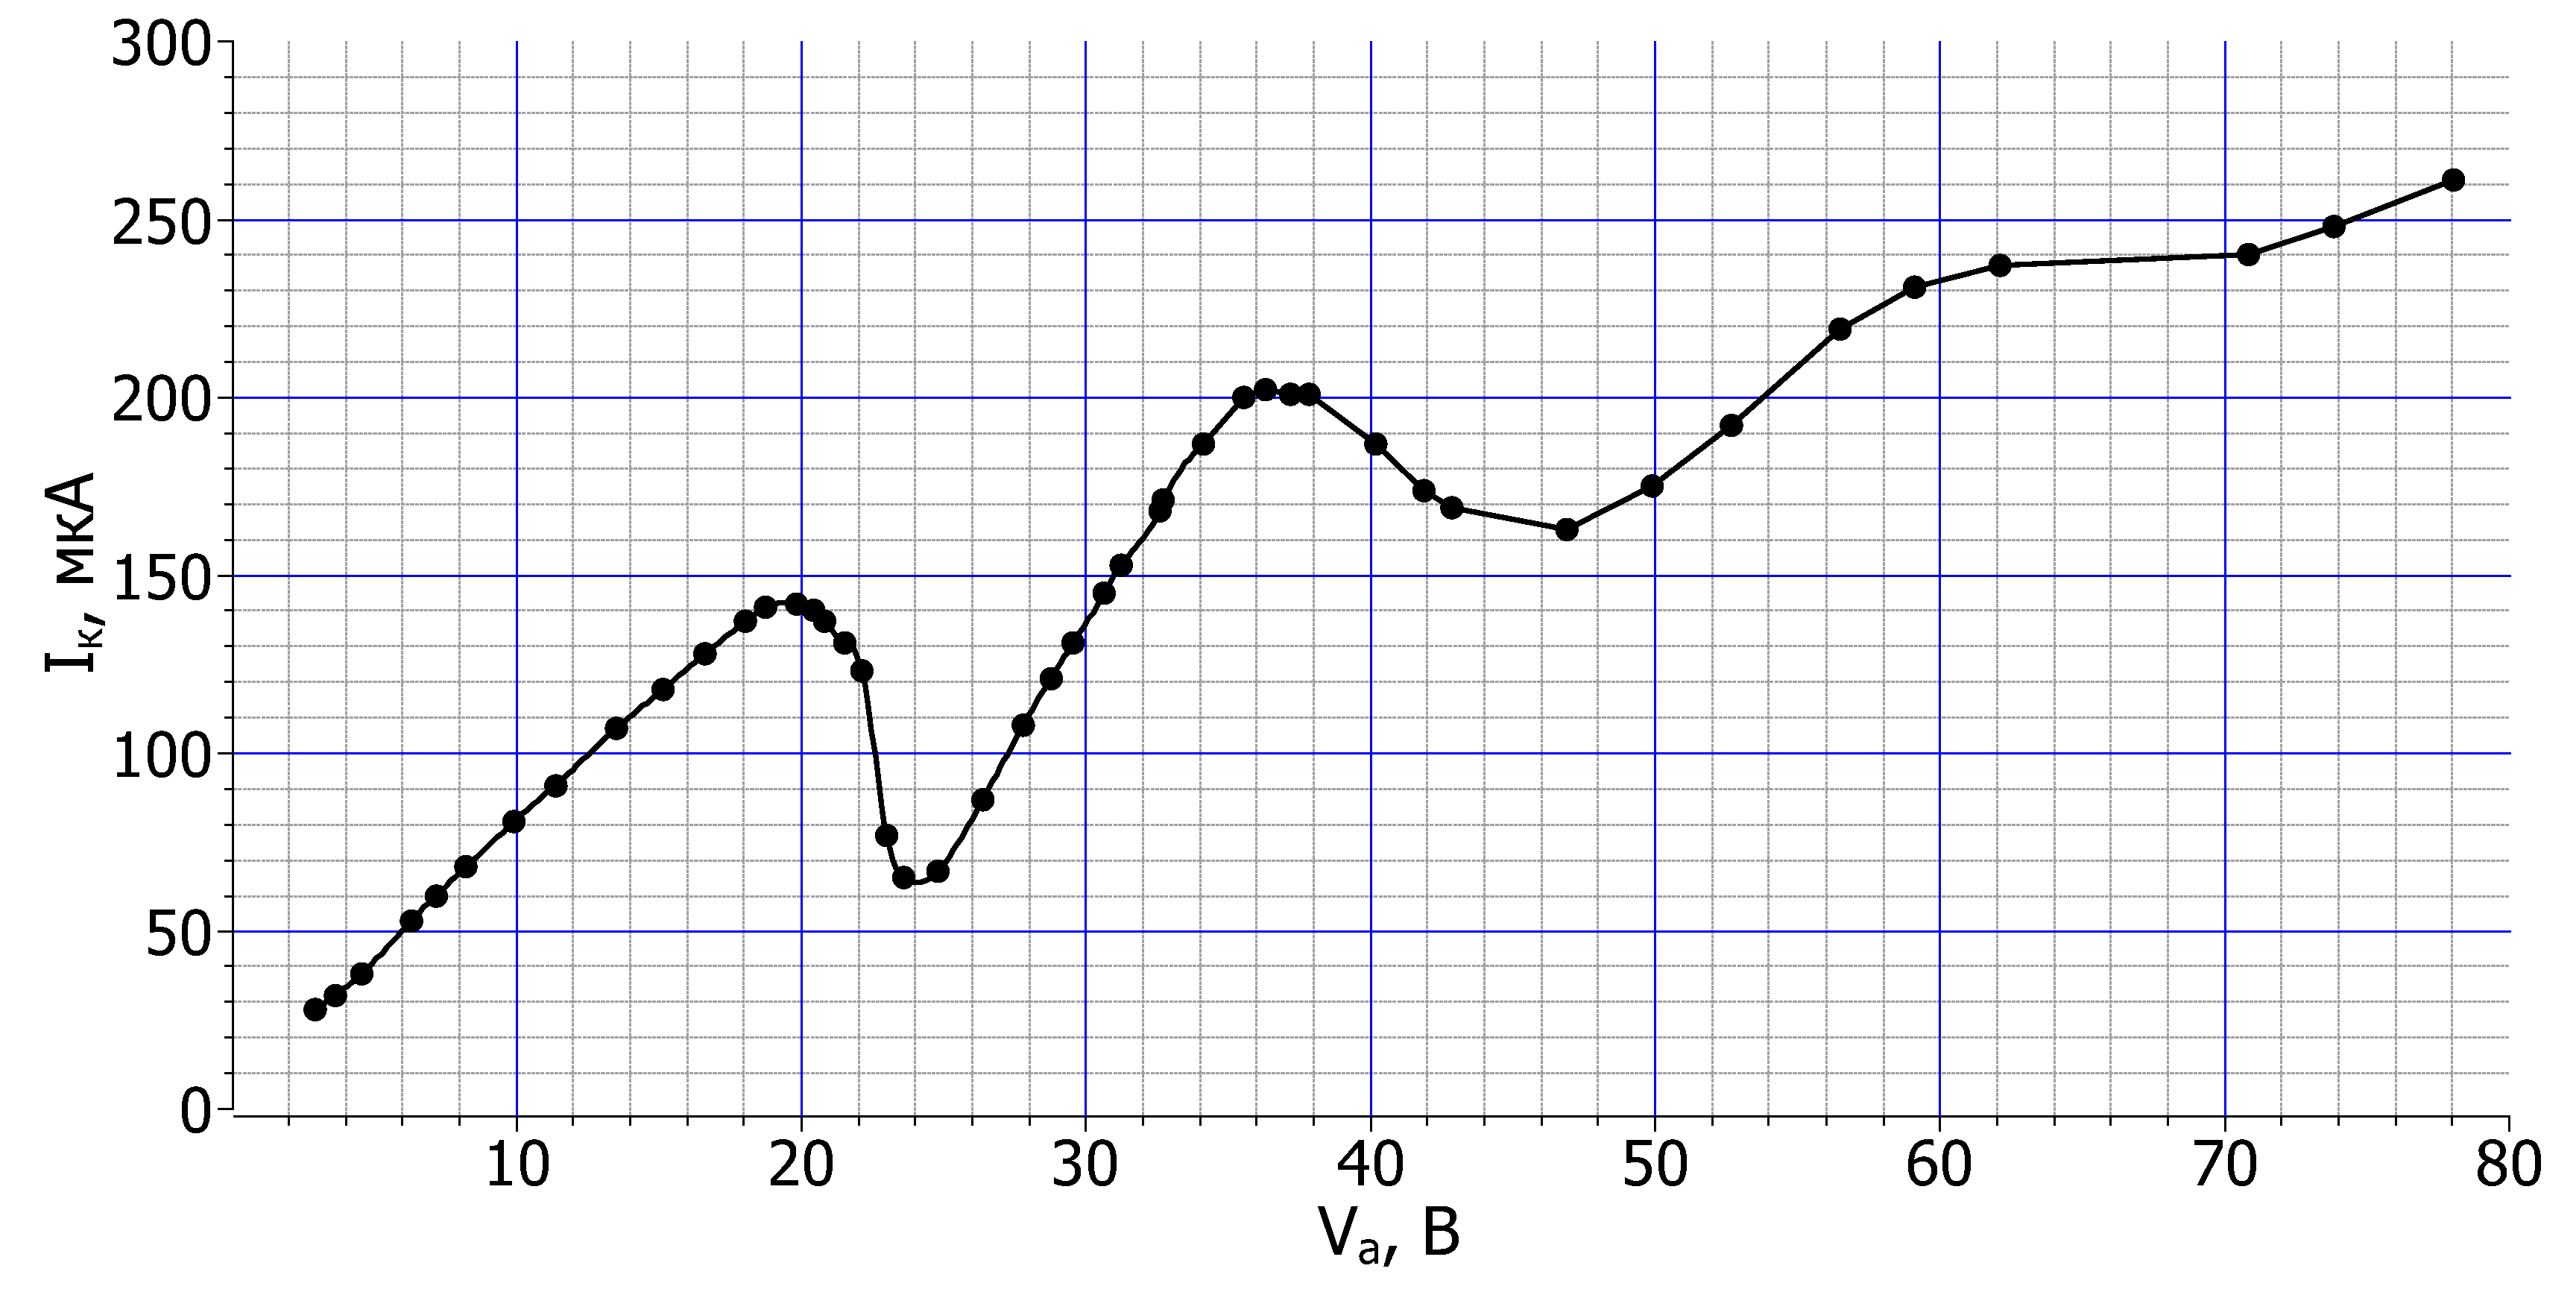
\includegraphics[width=\linewidth]{./Pictures/I(V)_4V}
 			\caption{Зависимость $I_\text{к}(V_a)$ при задерживающем напряжении 4 В}
 		\end{figure}
 	
 	
 		По графику находим:
 		\begin{equation*}
 			\Delta V = (21,72 \pm 0,07) \text{ В}
 			\hspace{20mm} (\text{погрешность}\thicksim 0,3 \% )
 		\end{equation*}
 	
 		Такая высокая точность достигается благодаря вольтметру и амперметру, которые в данном случае имеют погрешности 0,01 В и 1 мкА соответственно.
 		
 		
 		\begin{figure}[h!]
 			\centering
 			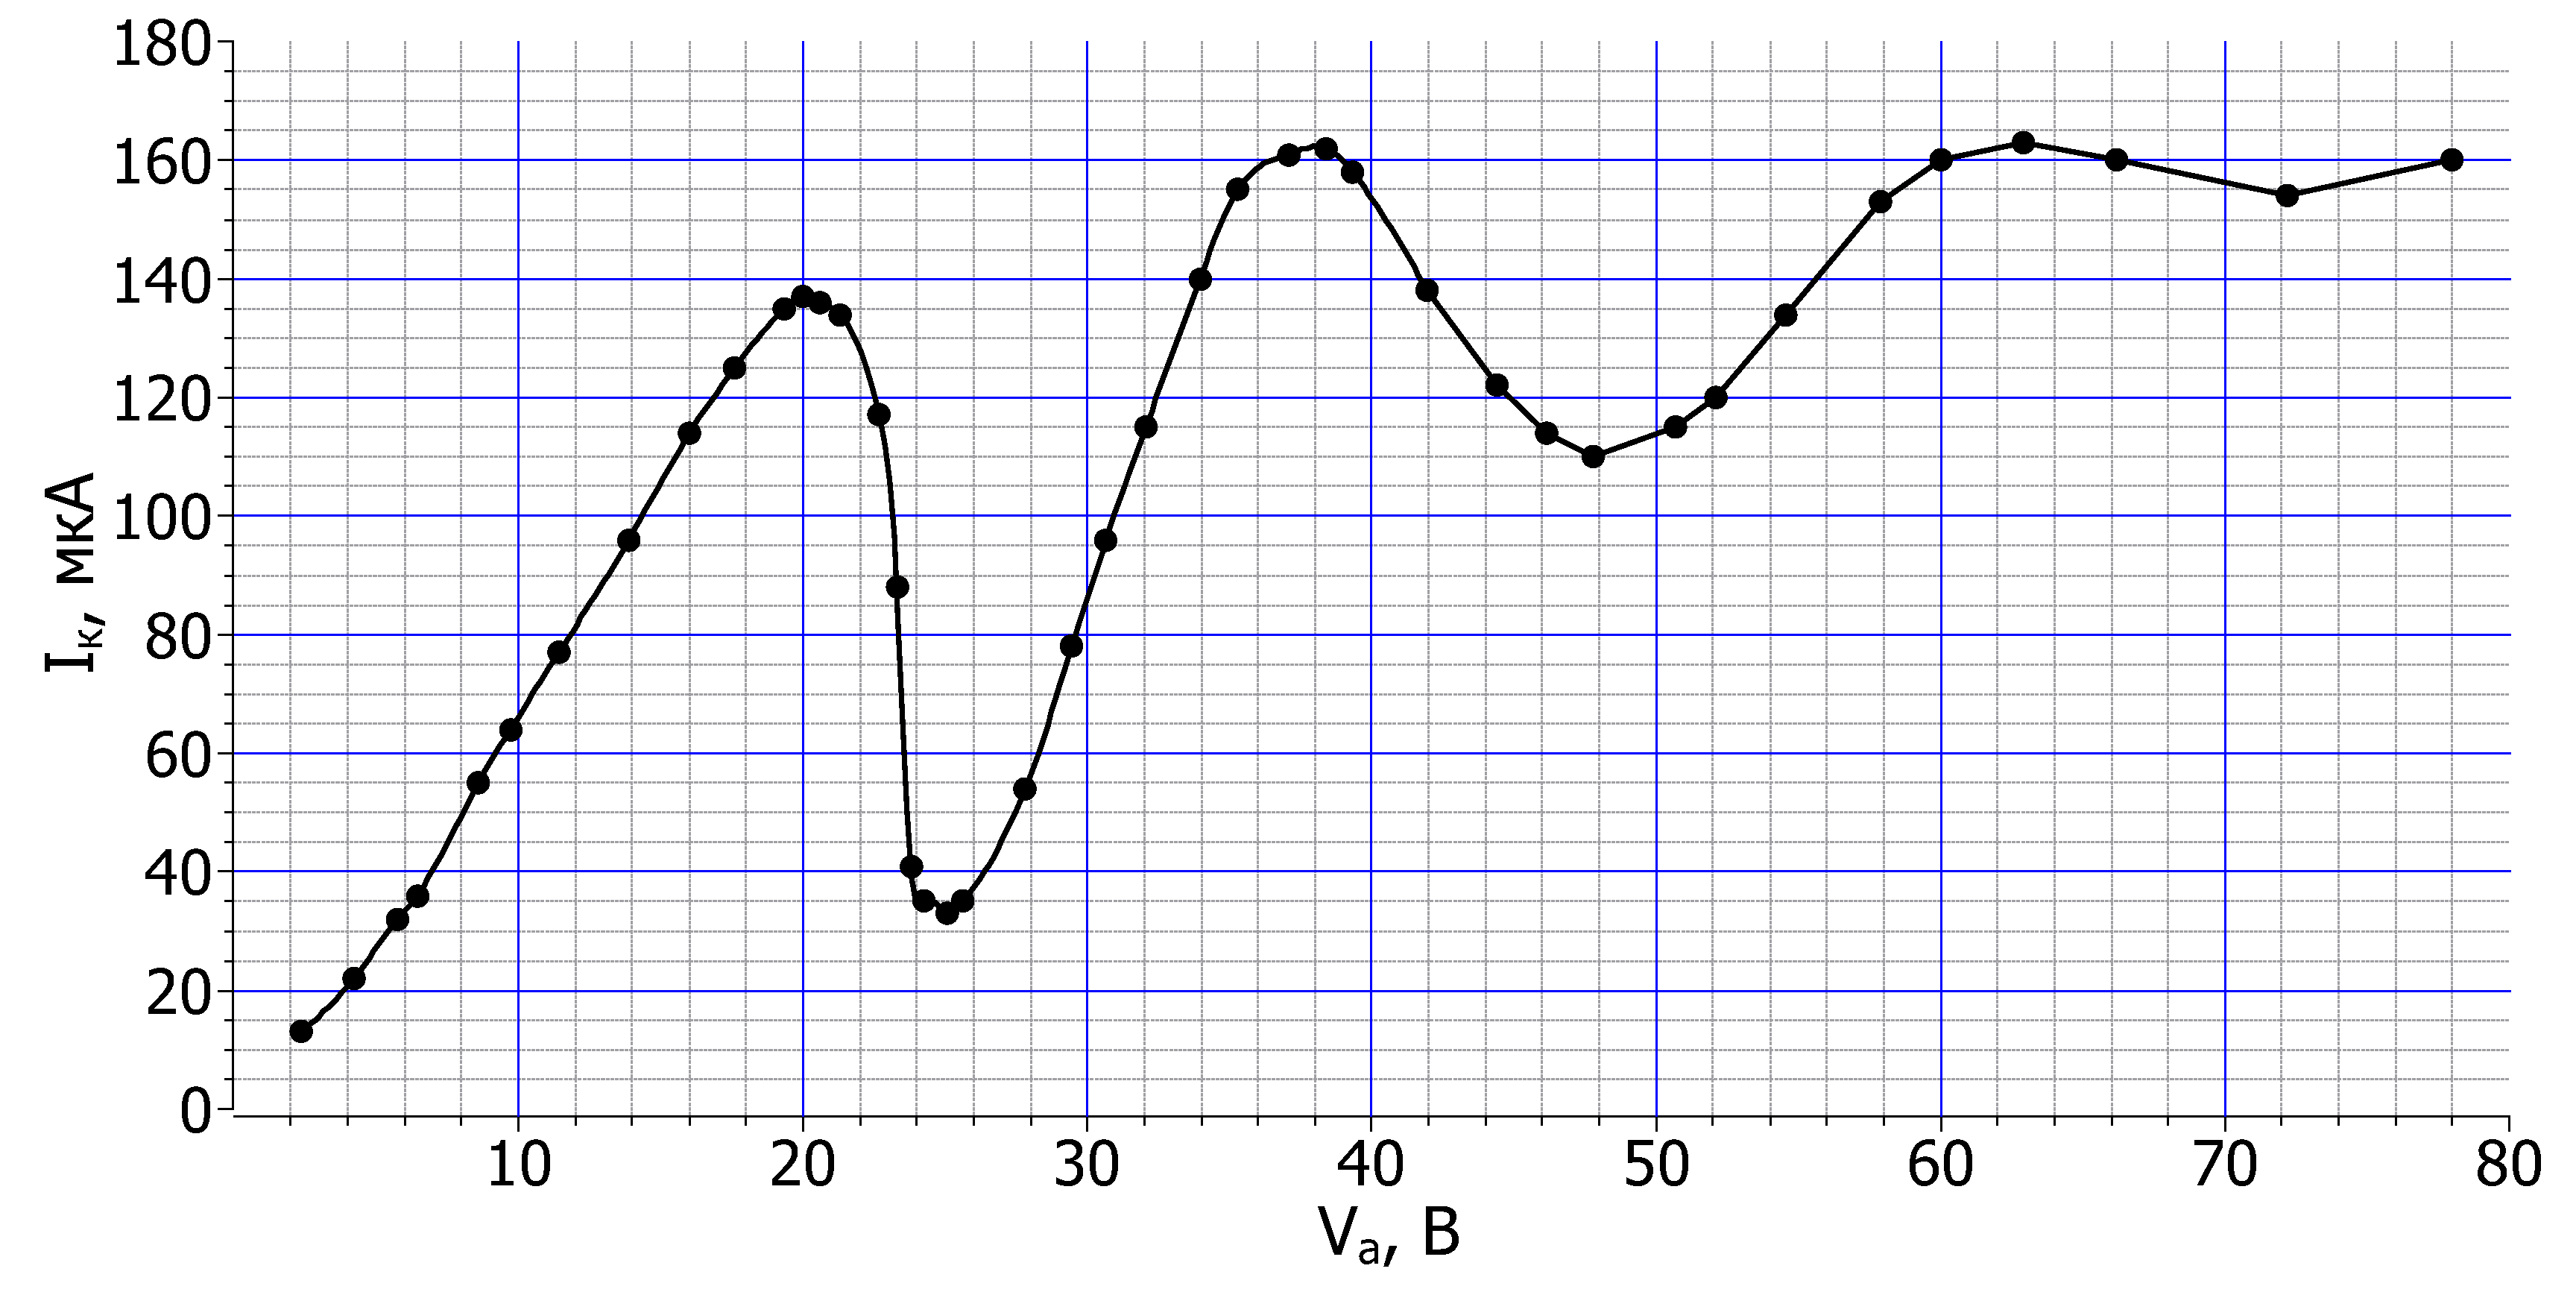
\includegraphics[width=\linewidth]{./Pictures/I(V)_6V}
 			\caption{Зависимость $I_\text{к}(V_a)$ при задерживающем напряжении 6 В}
 		\end{figure}
 		
 		
 		По этому графику находим:
 		\begin{equation*}
 			\Delta V = (21,89 \pm 0,09) \text{ В}
 			\hspace{20mm} (\text{погрешность}\thicksim 0,4 \% )
 		\end{equation*}
 	
 	
 		\begin{figure}[h!]
 			\centering
 			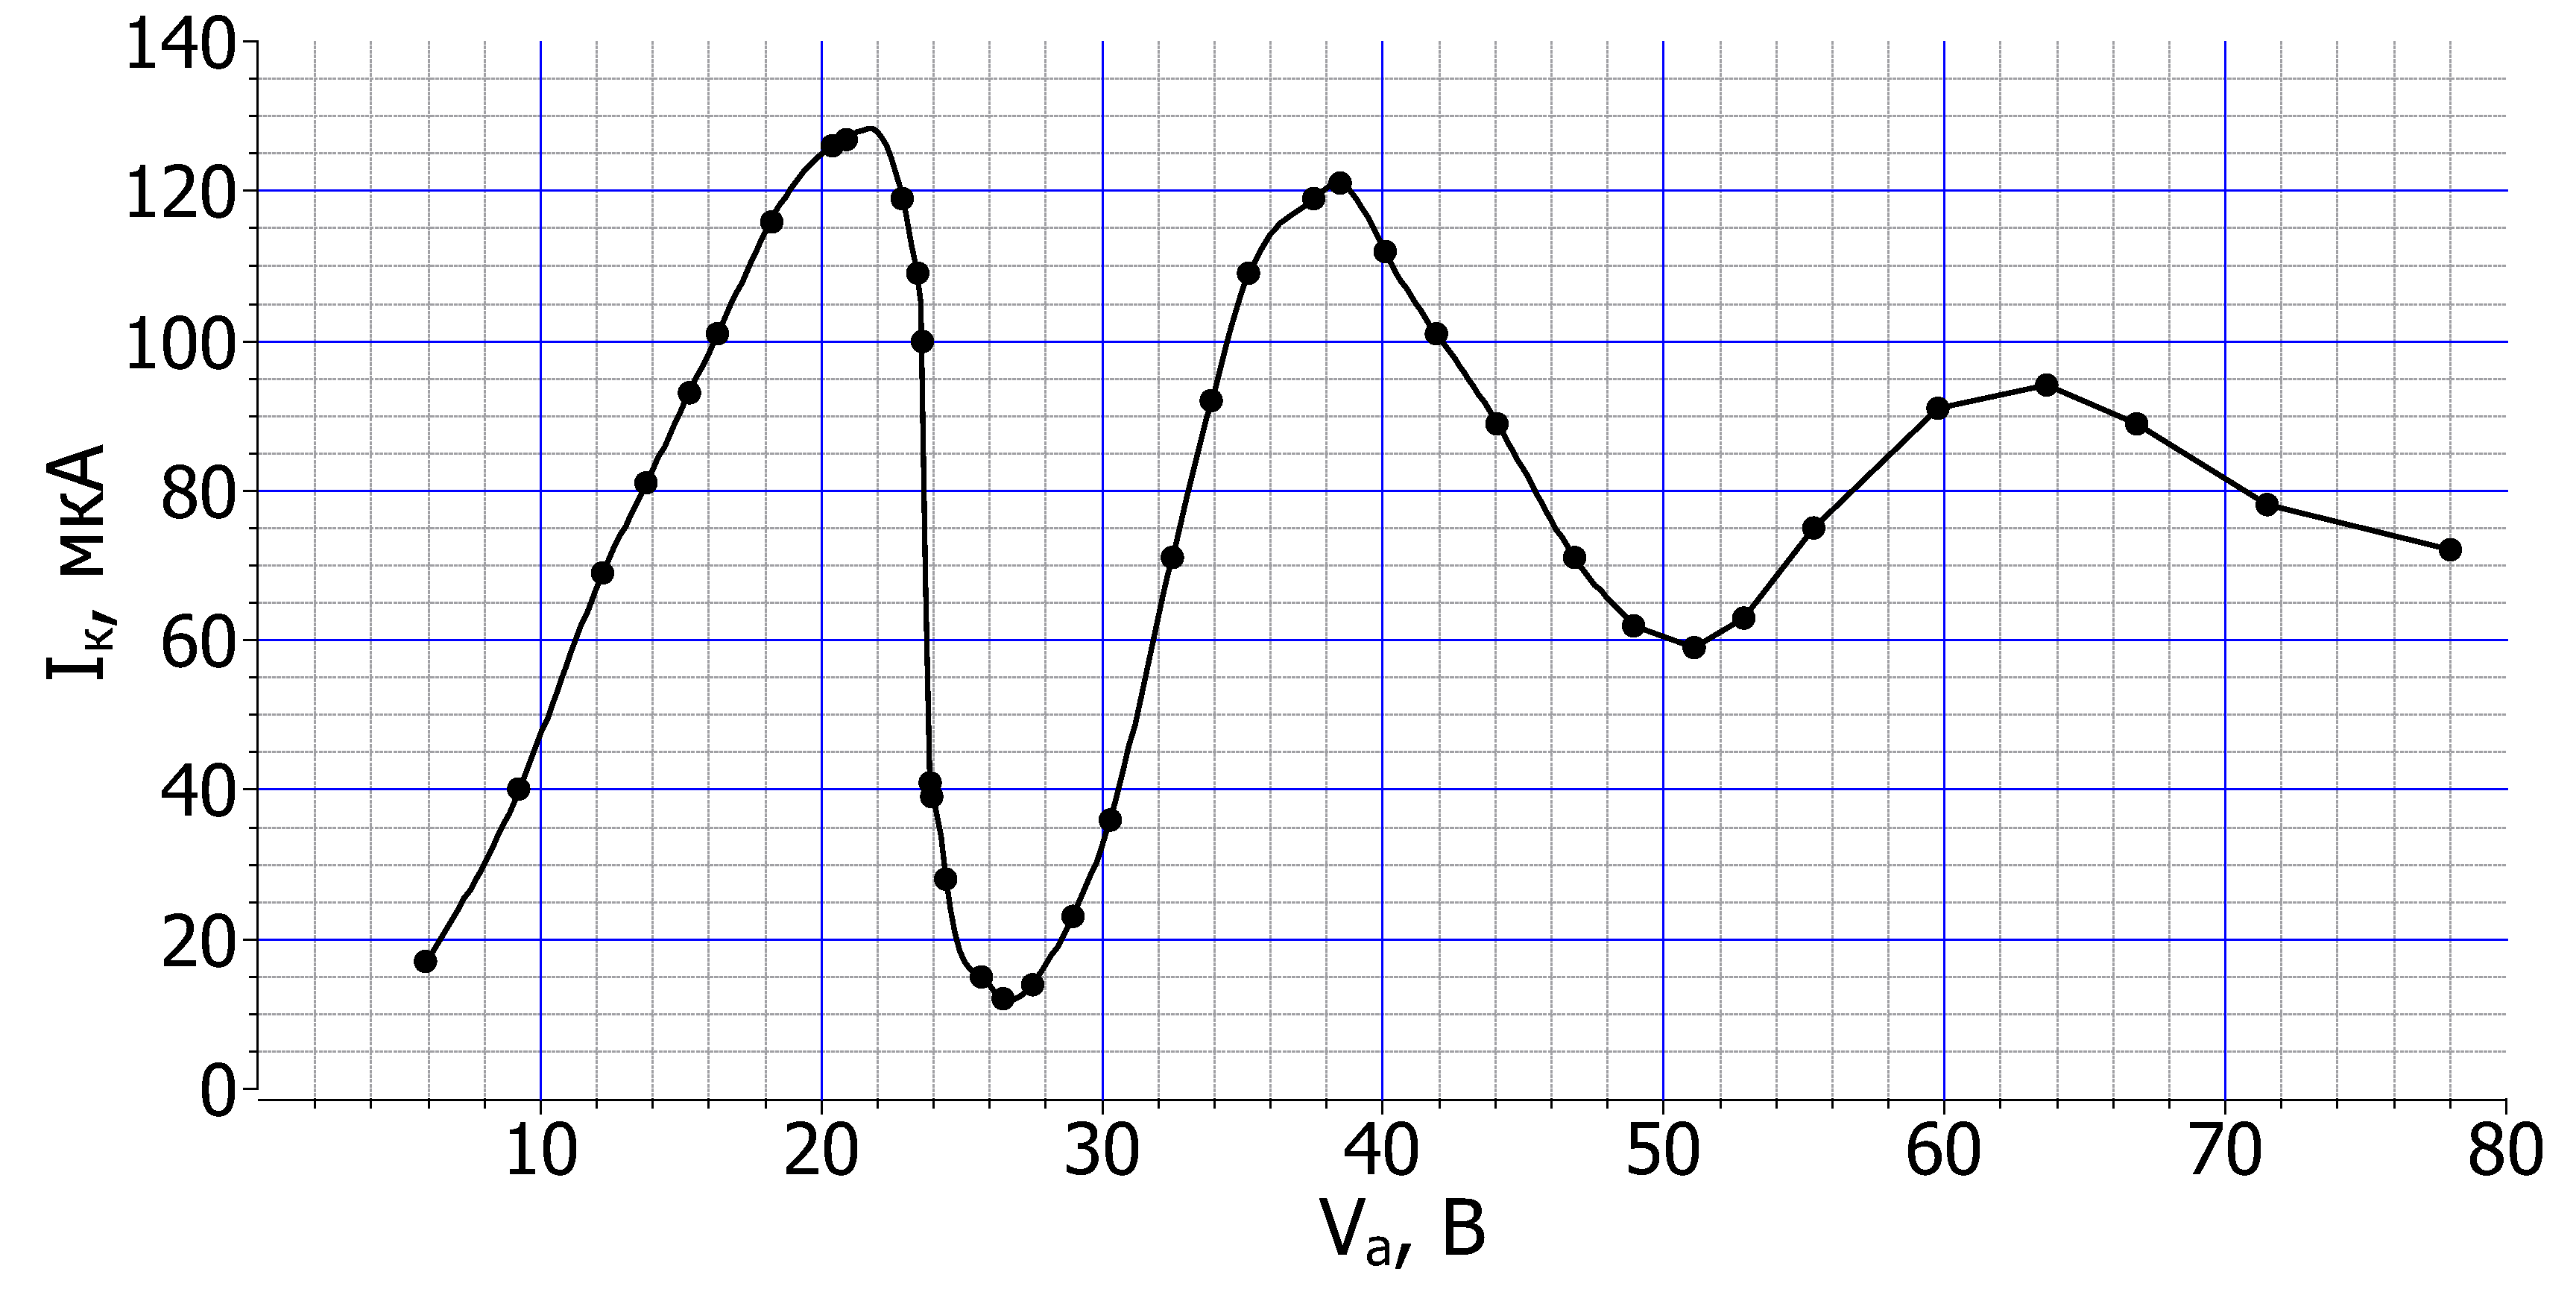
\includegraphics[width=\linewidth]{./Pictures/I(V)_8V}
 			\caption{Зависимость $I_\text{к}(V_a)$ при задерживающем напряжении 8 В}
 		\end{figure}
 		
 		
 		По данному графику находим:
 		\begin{equation*}
 			\Delta V = (22,0 \pm 0,2) \text{ В}
 			\hspace{20mm} (\text{погрешность}\thicksim 0,9 \% )
 		\end{equation*}
 	
 		И если посчитать среднее значение по этим трем графикам, то получим:
 		\begin{equation*}
 			\boxed{\Delta V^\Sigma = (21,9 \pm 0,3) \text{ В}}
 		\end{equation*}
 	
 		А значит, энергия возбуждения первого уровня атома гелия равна:
 		\begin{equation*}
 			\boxed{E_1^\Sigma = (21,9 \pm 0,3) \text{ эВ}}
 		\end{equation*}
 	
 		Погрешность составляет $\thicksim 1,4 \%$.
 		
 		\item В итоге мы наблюдаем такую картину: значения, полученные при динамическом и статическом методах достаточно сильно разнятся. Однако и погрешность у динамического метода велика -- около 23\%. Статический метод оказался гораздо лучше в плане точности -- его погрешности порядка всего лишь процента.
 		
 		Вдобавок, значение, вычисленное при статическом методе, оказывается чрезвычайно близко к табличному значению в 21,6 эВ, что даже укладывается в полученный интервал для $E_1$.
 	
 	\end{enumerate}
 
 	
 	\newpage
 	\tocsection{Вывод}
 	
 	В данной работе мы воспроизвели опыт Франка-Герца, который подтверждает наличие дискретных уровней возбуждения атомов. Опыт был проведен в динамическом и статическом режимах, из которых были получены следующие результаты для энергии возбуждения первого уровня атома гелия:
 	\begin{itemize}
 		\item $E_\text{dynamic} = (15,0 \pm 3,5) \text{ эВ} \hspace{20mm} (\text{погрешность}\thicksim 23 \% )$
 		
 		\item $E_\text{static} \;\;\; = (21,9 \pm 0,3) \text{ эВ} \hspace{20mm} (\text{погрешность}\thicksim 1,4 \% )$
 	\end{itemize}
 	Причем табличное значение $E = 21,6$ эВ. Как видим, статический метод дает очень близкое к нему значение и даже в пределах погрешностей совпадает. Динамический метод имеет куда большую ошибку, а также дает результат, находящийся гораздо дальше от табличного.
 	
 	Ошибка динамического метода связана с несовершенством техники измерения. Погрешности при статическом методе все же имеют куда меньшие значения благодаря точности вольтметра и амперметра. В контексте этой работы, процентаж ошибки этих приборов составляет всего лишь $\thicksim 0,1-3\%$.
 	
 
	
\end{document}